\chapter{Projective planes}

Some may already encountered the projective planes or at least their finite versions. In this chapter we will recall the definition and also some properties they have.

\section{Basics}

\begin{defn}
	Projective plane is hypergraf $(X, \mathcal{M})$ such that
	
	\begin{enumerate}
		\item every two (different) edges (or lines) intersect in exactly 1 point,
		\label{projective-plane-1st}
		\item for every 2 (distinct) points there exist exactly one edge containing them, \label{projective-plane-2nd}
		\item there are four points so no 3 of them lies on same edge. \label{projective-plane-3rd}
	\end{enumerate}
\end{defn}

\noindent One of the most well known finite projective plane is Fano plane, which can be seen on a picture \ref{fano-plane}.

\begin{figure}[!h]\centering
	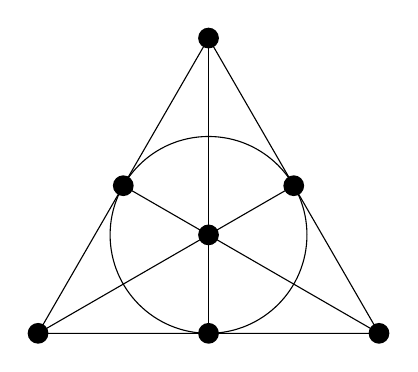
\begin{tikzpicture}[scale=2.5]
		\draw (0,0) circle (0.5);
		\draw (90:1) -- (-30:1)--(210:1)--cycle;
		\draw (90:1)--(0,0);
		\draw (210:1)--(0,0);
		\draw (-30:1)--(0,0);
		\draw (30:0.5)--(0,0);
		\draw (150:0.5)--(0,0);
		\draw (270:0.5)--(0,0);
		\fill (-0.866,-0.5) circle (1.5pt);
		\fill (0.866,-0.5) circle (1.5pt);
		\fill (0,-0.5) circle (1.5pt);
		\fill (0,1) circle (1.5pt);
		\fill (0,0) circle (1.5pt);
		\fill (0.433,0.25) circle (1.5pt);
		\fill (-0.433,0.25) circle (1.5pt);
	\end{tikzpicture}
	\caption{Fano plane.}
	\label{fano-plane}
\end{figure}

\begin{example}
	Now what about euclidean space $\R^2$? We can obviously see that part \ref{projective-plane-3rd} is satisfied, and also the property \ref{projective-plane-2nd}. Only for the very first one \ref{projective-plane-1st} we may encounter two lines which are parallel, hence they do not share any point. But we may establish an infinite point for which all such parallel lines in this direction go to. Therefore we must create a lot of infinite points, for every possible direction. But with such augmentation we have broken the property \ref{projective-plane-2nd} and so we need to add a line which goes through all infinite points.\label{r2-creation}
\end{example}

\section{Construction of projective planes}

As in the example \ref{r2-creation} shown before we will furthermore establish general technique to create a projective plane. Firstly in a geometric way and later on also in algebraic way.

Lets firstly start by taking 4 points, so we are trying to create a smallest possible finite projective plane. To fulfil all properties lets add few lines and end up with a box having two diagonals, see picture \ref{fano-plane-start}. Now we encounter the same problem as it was before, so we also add infinite points and extend the lines to them and also creating a line going through all of such infinite points. Note that \textit{parallel lines} now are those lines which don't cross each other in a point. With this procedure we get the following picture \ref{fano-plane-end} and we may see that it is indeed isomorphic to the well known Fano plane.

\begin{figure}[!h]\centering
	\begin{subfigure}{0.4\textwidth}\centering
		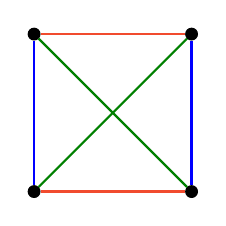
\begin{tikzpicture}[n/.style = {draw, circle, fill, inner sep=1.5pt}]
			\node[n] (1) at (0,0) {};
			\node[n] (2) at (0,2) {};
			\node[n] (3) at (2,0) {};
			\node[n] (4) at (2,2) {};
			\draw[color=Blue, thick] (1) to (2);
			\draw[color=Blue, thick] (3) to (4);
			\draw[color=Green, thick] (2) to (3);
			\draw[color=Green, thick] (1) to (4);
			\draw[color=RedOrange, thick] (1) to (3);
			\draw[color=RedOrange, thick] (2) to (4);
		\end{tikzpicture}
		\caption{Starting box with 6 lines and 4 points.}
		\label{fano-plane-start}
	\end{subfigure}
	\begin{subfigure}{0.4\textwidth}\centering
		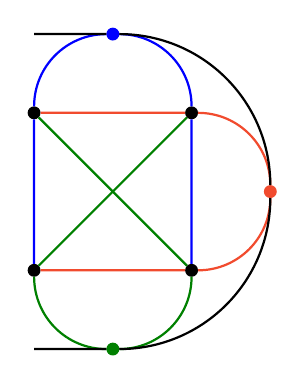
\begin{tikzpicture}[n/.style = {draw, circle, fill, inner sep=1.5pt}]
			\node[n] (1) at (0,0) {};
			\node[n] (2) at (0,2) {};
			\node[n] (3) at (2,0) {};
			\node[n] (4) at (2,2) {};
			
			\node[n, RedOrange] (i1) at (3,1) {};
			\node[n, Blue] (i2) at (1,3) {};
			\node[n, Green] (i3) at (1,-1) {};
			
			\draw[color=Blue, thick] (1) to (2) to[out=90, in=180] (i2);
			\draw[color=Blue, thick] (3) to (4) to[out=90, in=0] (i2);
			\draw[color=Green, thick] (2) to (3) to[out=270, in=0] (i3);
			\draw[color=Green, thick] (4) to (1) to[out=270, in=180] (i3);
			\draw[color=RedOrange, thick] (1) to (3) to[out=0, in=270] (i1);
			\draw[color=RedOrange, thick] (2) to (4) to[out=0, in=90] (i1);
			
			\draw[thick] (0,-1) to (i3) to[out=0, in=270] (i1) to[out=90,in=0] (i2) to (0,3);
		\end{tikzpicture}
		\caption{Ending with 7 lines and 7 points.}
		\label{fano-plane-end}
	\end{subfigure}
	\caption{Generating smallest projective plane.}
\end{figure}

We can also apply to this to other starting points. We may see the result of applying to $3 \times 3$ grid of points and resulting in a projective plane depicted on picture \ref{3by3}.

\begin{figure}[!h]\centering
	\begin{tikzpicture}[scale=1]
		\foreach \j in {1,...,3} {
			\foreach \i in {1,...,3} {
				\node[draw, circle, fill, inner sep=1.5pt] (\j-\i) at (2*\j,2*\i) {};
			}
		}
	\end{tikzpicture}
\caption{Creating a projective plane from $3 \times 3$ grid.}
	\label{3by3}
\end{figure}

But now one question may arise. In all cases we set few parallel lines and mainly decided which lines are so called \textit{diagonal}. Lets now generate such planes by using algebraic methods.

\subsection{Construction by algebraic methods}

Lets have $\mathbb{F}$ as a finite field. For such field we would like to create a projective plane. There are few approaches. We will show two of them.

\begin{enumerate}
	\item Take a vector space $\mathbb{F}^2$; that is tuples of elements from $\mathbb{F}$. The main lines are obviously those which are of a type $(c,x)$ and $(x,c)$ where $c$ is some element from $\mathbb{F}$ and $x$ is increasing elements from the same field. And the diagonals are such lines which has the same difference between the two points, or in other words the same \textit{slope}.
	
	\item Lets now take a vector space $\mathbb{F}^3$. Now the points are (sub)spaces of dimension 1; and the lines are (sub)spaces of dimension 2. Therefore points are lines and lines are planes. Therefore all properties \ref{projective-plane-1st}, \ref{projective-plane-2nd} and \ref{projective-plane-3rd} are satisfied from the perspective of linear algebra.
\end{enumerate}

\section{Further definitions and observations}

Lets talk about some other propositions and definitions of projective planes.

\begin{defn}
	Order of projective plane is the number of points on every line $-1$.
\end{defn}

For this definition it is crucial to show that each line has the same number of points. For this see the next lemma.

\begin{lemma}
	Every projective plane has all lines of same size.
\end{lemma}

\begin{proof}
	When we have two different lines $p,q$ and a point $x$ not lying on any of those, then we set a bijection of points from $p$ to points from $q$ by the lines derived from $x$ and the point of $p$. Since all such lines intersect in a common point $x$ then they cannot intersect in any point of $q$.
	
	Note that the existence of such $x$ is not obtained by default. Either it exists from the property \ref{projective-plane-3rd}. If all points from this property are on $p$ or $q$ it must happen that exactly two of them are on $p$ and the rest on $q$ thus seeing a lines going through these four points we get a common meeting point, which will be our desired $x$.
\end{proof}

Now one can already see that if we take projective planes of order $2$ we have $2 \cdot 2 + 2 + 1$ points and for order $3$ we have $3 \cdot 3 + 3 + 1$. So that the next proposition is true.

\begin{prop}
	Projective plane of order $n$ has $n^2 + n + 1$ points.
\end{prop}

\begin{proof}
	Lets take a line $p$ and a point $x$, for every point on $p$ (where there is $n+1$ of them) we see the line going through $x$ and such point. On all of these lines there is another $n-1$ points. Therefore in total we have $n+1 + (n+1) \cdot (n-1) +1 = n^2 + n +1$.
	
	Also note that we haven't missed any of the points. Otherwise there is a path going through $x$ and such point and this line must intersect $p$ in one point, therefore it was already considered.
\end{proof}

Lastly see the table of known results.

\begin{table}[!h]\centering
	\begin{tabular}{c | c | c | c | c | c | c | c | c | c | c}
		2 & 3 & 4 & 5 & 6 & 7 & 8 & 9 & 10 & 11 & 12 \\
		Fano plane & Shown & & No plane in 1900. & & & & & Computer search. & & OPEN
	\end{tabular}
\end{table}